\documentclass[12pt]{article}
\usepackage{shortex}
\usepackage{qp}
\usepackage[margin=1in]{geometry}
\usepackage{tikz}
\usepackage{longtable}
\usepackage{cite}
\usetikzlibrary{arrows.meta}
\author{Zachary Lau}
\title{A Critique and Simulation Study on Extended Ensemble Kalman Methods}
\date{\today}

\begin{document}
\maketitle

\begin{abstract}
Traditional inference methods for state-space models work well when the dimension is
low or under normality assumptions on the latent state and the data-generating
process. However, they break down when both assumptions are violated. Recent
research has proposed performing inference for such models by combining ensemble
Kalman filter (EnKF) methods with sequential Monte Carlo (SMC) methods. In this
qualifying paper, we provide a critique of existing methods, and of related
experiments found in the literature. Furthermore, we perform a simulation study
to address these experimental gaps. Our main theoretical critique concerns the
practicality of implementing these algorithms. Despite these limitations,
experimental evidence from our simulation study shows that when these algorithms
can be implemented, they are effective tools for inference under non-normality
and a moderately high-dimensional latent state ($d=100$), and successfully avoid
the extreme weight-degeneracy found with a naive SMC approach. A proposed
extension involves using the EnKF as a proposal distribution within an SMC
framework to ensure asymptotic consistency. This is in contrast to existing
methods which treat the EnKF as an exact sampling method, even when this may not
be true.
\end{abstract}

% Problem setup
\section{Introduction}
State-space models are a widely applied and useful tool whenever we are
modelling the evolution of some sort of state over time, given observations
which are dependent on the underlying state. Examples include modelling
the behaviour of animals given tracking data, the location
of a plane given radar readings, or the state of a climate system given
observations at a set of weather stations.

The classical frequentist approach
to estimating a continuous state is the Kalman filter \cite{kalman1960,simon2006}. This
method starts with an initial estimate of the state, as well as a
quantification of the uncertainty of that estimate. The estimate and uncertainty
quantification are iteratively used to forecast the next step, and then
updated based on observations from that time step. However, the basic
Kalman filter only applies when our physical model is linear, and noise
is Gaussian. This makes it difficult to account for non-linear effects. For example,
we cannot account for pitch, yaw and roll in the vehicle dynamics model.
The extended Kalman filter addresses this problem by using non-linear dynamics
for the forecasting step, but using a linearized model to update the forecast
covariance \cite{jazwinski1970,evensen2009}. Extended Kalman filters work well for low-dimensional problems.
However, they may suffer from two main problems. Firstly, the covariance
updates remain inexact, which may cause instability \cite{evensen1992}.
Furthermore, when the state space is high dimensional, it becomes extremely
costly to propagate and update a dense covariance matrix. This problem
inspired the ensemble Kalman filter (EnKF) \cite{evensen1994,evensen2003}.
The EnKF addresses these issues by maintaining a particle
approximation of the filtering distribution. Crucially, the number of particles
required for an accurate representation of the distribution is often much lower
than the dimension of the state space. This enables a low-rank representation
of the covariance matrix.

The EnKF represents the state of the art for high-dimensional
climate-based state-space models. However, it is still constrained by the
Gaussian constraints on the observation noise and the modelling noise introduced
during the forecasting steps. This restraint restricts us, for example, from
performing inference on models with skewed or heavy-tailed distributions such as
rainfall. In low dimensions, these scenarios can be approached by Markov chain
Monte Carlo (MCMC), sequential Monte Carlo (SMC) methods
\cite{doucet2001,doucet2000,chopin2020} or mixture Kalman filters
\cite{chen2000}. These methods also work by propagating an ensemble of
weighted particles through time, but are more capable of dealing with
non-normality. Unfortunately, in high dimensions these techniques are known to
suffer from weight-degeneracy, wherein a single particle is assigned all of the
weight of the ensemble, which degrades the quality of inference and makes them
useless for estimating uncertainty.

\section{Methodology}

\subsection{The Gibbs and particle ensemble Kalman filters}
In \cite{katzfuss2020} the authors propose combining ensemble Kalman methods
with SMC methods, in the Gibbs ensemble Kalman filter (GEnKF) and the particle
ensemble Kalman filter (PEnKF). In this work, the state is divided into two parts,
a high-dimensional part which is well modelled by Gaussian model dynamics,
and a low-dimensional part which is not modelled well by Gaussian dynamics.
For example, the high-dimensional section may consist of a large spatial grid,
whereas the low-dimensional part of the state space may consist of a set of
parameters over which we wish to perform Bayesian inference. Their key
algorithmic contribution is to use an EnKF to propagate
uncertainty about the high-dimensional portion of the state, while using SMC 
and MCMC techniques to account for non-Gaussian posteriors over specific
parameters, or in the noise distribution. This reduces the effective
dimensionality of the SMC problem, allowing one to incorporate both
high-dimensional latent spaces, as well as non-Gaussian parameters -- a
combination previously inaccessible to either SMC methods or EnKF methods on
their own.

\subsubsection{Hierarchical state-space models}
The generic hierarchical state-space model (HSSM) considered in \cite{katzfuss2020} is
shown below.
\begin{align}
    \theta_t \mid \theta_{t-1} &\sim p(\theta_t \mid \theta_{t-1}) \label{eq:prior}\\
    \vx_t \mid \vx_{t-1}, \theta_t &\sim \Norm_d(\mathcal M_t(\vx_{t-1}; \theta_t), \mathbf Q_t) \\
    \vy_t \mid \vx_t, \theta_t &\sim \Norm_{m_t}(\mathbf H_t \vx_t, \mathbf R_t) \\
    \vz_t \mid \vy_t, \theta_t &\sim f_t(\vz_t \mid \vy_t, \theta_t) \label{eq:transform}
\end{align}
This model extends that in which Kalman filtering is typically applied by
introducing a non-Gaussian parameter in Equation~\eqref{eq:prior}, and a transformation
which can account for non-normality in the observations in Equation~\eqref{eq:transform}.
Due to these extensions, a traditional EnKF is inappropriate.
However, when the dimension of $\vx$ is very high, such as a large spatial grid,
then SMC methods will suffer from weight-degeneracy.

\begin{example}[Rainfall model]\label{ex:rainfall}
A practical example of such an HSSM is the rainfall
model provided in \cite{katzfuss2020} and based on 
\cite{sanso1999} and \cite{sigrist2012}. This model is shown below
\begin{align}
    \theta_t &\sim p(\theta_t) \\
    \vx_t \mid \vx_{t-1} &\sim \Norm_d(\mathcal M_t(\vx_{t-1}), \mathbf Q_t) \\
    \vy_t \mid \vx_t &\sim \Norm_{m_t}(\mathbf H_t \vx_t , \sigma^2_t \mathbf I_{m_t})  \\
    z_{t,l} \mid \vy_t ,\theta_t &= y_{t,l}^{\theta_t} \1_{\{y_{t,l} > 0\}}, \quad l = 1, \ldots, m_t 
\end{align}
This model reflects a large group of locations with spatially correlated
rainfall, and a series of stations at some, but not all, locations. Furthermore,
the rainfall at all locations is modulated by a time-dependent global parameter
$\theta_t$. Our high-dimensional latent state in this example is $\vx$.
\end{example}

\subsubsection{PEnKF}
The most basic method proposed by \cite{katzfuss2020} is the
PEnKF. This algorithm maintains a
particle representation of the filtering distribution of $\theta_t$, as well as 
one ensemble for each $\theta_t$. The algorithm is described as follows
\begin{enumerate}
    \item Initialize a set of $N$ particles from the prior $p(\theta_0)$ with weights
    $w^i = \frac 1 N$ and for each $\theta_0^i$ an ensemble of $M$ particles
    $\vx_0^{ij} \sim \Norm_d(\boldsymbol\mu_{0|0}, \mathbf\Sigma_{0|0})$
    \item For each time step $1, \ldots, T$
    \begin{enumerate}
        \item For each particle $i = 1, \ldots, N$
        \begin{enumerate}
            \item Sample from a proposal $q_t(\theta^i_t \mid \theta^i_{t-1})$
            \item Propagate the ensemble. That is, compute the \emph{forecast}
            by applying the model to each ensemble member,
            $\tilde \vx^{ij}_{t} := \mathcal M_t(\vx^{ij}_{t-1}; \theta_t^i)$
            for $j = 1, \ldots, M$
            \item Update particle weights
            \begin{align}
                w^i_t \propto w^i_{t-1}\mathcal L_t(\vz_t \mid \theta_t^i, \tilde\vx^{i,1:M}_t)
                p(\theta_t^i \mid \theta_{t-1}^i)/q_t(\theta_t^i \mid \theta_{t-1}^i)
            \end{align}\label{step:likelihood}
            \item Draw a new ensemble $\vx^{ij}_t$ afresh from the conditional distribution
            $p(\vx^{ij}_t \mid \theta^i_{1:t}, \vz_{1:t})$ \label{step:sample}
        \end{enumerate}
    \end{enumerate}
    \item If desired, resample particles $\theta^i$ to rebalance weights.
\end{enumerate}
The major immediate challenges in making such an algorithm work include
estimating the likelihood term in step~\ref{step:likelihood}, and sampling from
the conditional distribution in step~\ref{step:sample}. In particular,
\cite{katzfuss2020} suggest using a normal approximation to the forecast
distribution $p(\tilde\vx^i_t \mid \vz_{1:t-1})$ based on an estimate of the mean
and covariance of the ensemble. \cite{katzfuss2020} also use the EnKF to perform
approximate sampling in step~\ref{step:sample}. Practically, we are also limited by
the number of $\theta$ particles $N$ we can use, since each particle requires
its own ensemble of $M$ further particles. The PEnKF avoids the weight
degeneracy problem by effectively only using SMC to model the filtering
distribution of $\theta$, which has much lower dimension.
% Suggested - use EnKF to approximate likelihood here

\subsubsection{GEnKF}
Under appropriate conditions on our model, the requirement for an ensemble of
ensembles can be relaxed, and instead a single ensemble can be used which
covers both $\vx_t$ and $\theta_t$. The required conditions are forecast
independence, and tractability of full conditional distributions (FCDs).

\begin{condition}[Forecast independence]\label{cond:forecast}
An HSSM is said to exhibit forecast independence if
\begin{align}
    p(\tilde\vx_t, \theta_t \mid \vz_{1:t-1}) &=
        p(\tilde\vx_t \mid \vz_{1:t-1})p(\theta_t \mid \vz_{1:t-1})
\end{align}
\end{condition}

\begin{condition}[Full conditional distributions]\label{cond:conditional}
An HSSM satisfies the FCD condition if we can
tractably sample from $p(\vy_t \mid \vx_t,\theta_t,\vz_{1:t})$ and 
$p(\theta_t \mid \vy_t, \vx_t, \vz_{1:t})$
\end{condition}

Condition~\ref{cond:forecast} is satisfied in relatively straightforward, but by
no means all-encompassing scenarios.  For example, it holds when the
$\theta_t$ are independent, and the forecasting model $\mathcal M$ does not
depend on $\theta_t$, as in Example~\ref{ex:rainfall}.
Figure~\ref{fig:hssm-dag} shows a partial causal graph for the HSSM, and elucidates how these conditions imply forecast
independence.  Condition~\ref{cond:conditional} is more complicated to verify,
and also less clear cut, as tractability of sampling depends on what inference
algorithm we are using. It is most straightforward to show in the case of conjugate
priors, as happens in Example~\ref{ex:rainfall} for the 
draw from $p(\vy_t \mid \vx_t, \theta_t, \vz_{1:t})$. The resulting
algorithm is described below.
\begin{enumerate}
    \item Sample an ensemble $(\vx^i_0, \theta^i_0)$ for $i=1,\ldots, M$
    from the prior at $t=0$
    \item For each time step $t = 1, 2, \ldots, T$
    \begin{enumerate}
        \item Compute the forecast ensemble $\tilde \vx^i_t = \mathcal M(\vx^i_{t-1})$ for
        $i=1,\ldots, M$
        \item For each particle $i=1, \ldots, M$ perform Gibbs sampling
        \begin{enumerate}
            \item Choose initial values for $\vy^i_t$ and $\theta^i_t$
            \item Until convergence
            \begin{enumerate}
                \item Sample $\vx^i_t$ by picking a random ancestor from $j=1$
                to $M$ and performing the EnKF update on
                $\tilde \vx^j_t$ given $\vy^i_t$ and $\theta^i_t$
                \label{step:enkf}
                \item Sample $\vy^i_t$ from $p(\vy^i_t \mid \theta^i_t, \vx^i_t, \vz_{1:t})$
                \item Sample $\theta^i_t$ from $p(\theta^i_t \mid \vy^i_t, \vx^i_t, \vz_{1:t})$
            \end{enumerate}
        \end{enumerate}
    \end{enumerate}
\end{enumerate}
A key variance reduction technique suggested by \cite{katzfuss2020} is to run
each chain in parallel, and to use systematic resampling \cite{chopin2020}
across chains in step~\ref{step:enkf}. The GEnKF avoids the weight degeneracy
problem by avoiding weights entirely and sampling directly from the filtering
distribution.

It is clear that Condition~\ref{cond:conditional} is necessary to make the Gibbs
sampler work.  Forecast independence is required because the EnKF update relies
on a sample-based estimate of the forecast covariance of $\tilde\vx_t$. Under
forecast independence, the distribution of $\tilde\vx_t$ is independent of
$\theta$, and therefore we can pool all elements of the ensemble to form this
estimate. Without forecast independence, the covariance would be dependent on
$\theta_t$, and we would require a new ensemble for every $\theta_t^i$, as in
the PEnKF, or a reweighting of the existing ensemble which is likely to suffer
from weight-degeneracy \cite{katzfuss2020}.

\begin{figure}[ht]
\centering
\begin{tikzpicture}[
    >={Stealth[length=2.5mm]},
    var/.style={circle, draw, minimum size=1.1cm, inner sep=1pt},
    obs/.style={rectangle, draw, minimum width=1.1cm, minimum height=0.9cm, inner sep=2pt},
    new/.style={red, thick},
    node distance=3cm
]
    % Time t-1
    \node[var] (th0) at (0,0) {$\theta_{t-1}$};
    \node[var] (x0)  at (0,2.8) {$\vx_{t-1}$};
    \node[var] (y0)  at (0,5.6) {$\vy_{t-1}$};
    \node[obs] (z0)  at (0,8.2) {$\vz_{t-1}$};

    % Forecast
    \node[var] (xf)  at (4.5,2.8) {$\tilde\vx_t$};

    % Time t
    \node[var] (th1) at (9,0) {$\theta_t$};
    \node[var] (x1)  at (9,2.8) {$\vx_t$};
    \node[var] (y1)  at (9,5.6) {$\vy_t$};
    \node[obs] (z1)  at (9,8.2) {$\vz_t$};

    % Time t-1 edges
    \draw[->] (th0) -- (x0);
    \draw[->] (x0) -- (y0);
    \draw[->] (y0) -- (z0);
    \draw[->] (th0) to[bend left=30] (y0);
    \draw[->] (th0) to[bend left=30] (z0);

    % Time t edges
    \draw[->] (th1) -- (x1);
    \draw[->] (x1) -- (y1);
    \draw[->] (y1) -- (z1);
    \draw[->] (th1) to[bend right=30] (y1);
    \draw[->] (th1) to[bend right=30] (z1);

    % Forecast edges
    \draw[->] (x0) -- (xf);
    \draw[->] (xf) -- (x1);

    % Parameter dynamics and parameter dependence of the forecast
    \draw[dashed, ->, new] (th0) -- (th1);
    \draw[dashed, ->, new] (th1) -- (xf);
\end{tikzpicture}
\caption{Causal graph of the HSSM. Observed
variables $\vz_t$ are drawn as squares. For forecast independence, we condition
on $\vz_{t-1}$, but not $\vz_t$. The edge from $\theta_t$
to $\tilde\vx_t$ comes from the influence of $\theta_t$ on the model
$\mathcal M$. A sufficient condition to induce forecast independence is to
remove this edge, as well as the back-door path through $\theta_{t-1}$.
The latter can be done by assuming $\theta_t$ and $\theta_{t-1}$ are independent.}
\label{fig:hssm-dag}
\end{figure}

\subsection{Criticism of existing literature and method}\label{sec:criticism}
The use of the EnKF within Bayesian state-space models is certainly a
powerful idea which deserves further investigation. It successfully attacks
the central question of weight-degeneracy in inference on state-space models,
although at the cost of introducing bias. Unfortunately, this method as it
currently stands is extremely difficult to actually implement.

Firstly, as the authors in \cite{katzfuss2020} mention, but do not emphasize,
the GEnKF has only been shown to be reasonably implementable under fairly
restrictive circumstances. For example, if we work in the framework of
Conditions~\ref{cond:forecast} and~\ref{cond:conditional}, we must abandon
very reasonable modelling choices such as using our parameter $\theta$ in
the dynamic model $\mathcal M$, or using the same $\theta$ over all time steps.
Furthermore, the authors fail to discuss the difficulty of actually sampling
from the conditional distributions $p(\vy \mid \vx,\vz,\theta)$ and
$p(\theta \mid \vx,\vy,\vz)$. Several problems may occur. Firstly, if $\vy$ is
moderately high dimensional and cannot be decomposed by dimensions, we still
have a nested high-dimensional sampling problem. Even if the
$y_l$ are independent and we have access to the conditional density, we generally will still need to
perform MCMC to sample from this density. As this is done inside the Gibbs
sampler, this becomes a nested MCMC. We face exactly the same problem sampling
from $p(\theta \mid \vx,\vy,\vz)$. The requirement for nested MCMC significantly
slows down the sampling procedure, and introduces many more tuning
parameters such as step sizes and numbers of iterations that must be chosen
wisely for effective inference. 

Furthermore, the experimental setup presented in \cite{katzfuss2020} has
several peculiar implementation details, and fails to address key scenarios of
interest. We first focus on their experiment on the rainfall model in
Example~\ref{ex:rainfall}.  The authors perform this experiment for both a
fixed, known, $\theta$ and an unknown $\theta$. One strange choice they make
in this experiment is to infer $\theta$ using state-augmentation. This method
incorporates $\theta$ into the state vector. However, doing so violates the
model requirement that $\theta > 1$. The authors make no effort to reconcile
this conflict. The second peculiarity about this experiment is that the
authors only perform the filtering update for a single time step. The intention
appears to be to isolate the effect of the ``update'' step in their algorithm.
Additionally, doing only a single update step allows them to develop a ground
truth for the posterior by running standard MCMC. However, in doing so they
remove many of the important aspects of the state-space model, such as
information sharing between time points, or potential non-linear effects of
the dynamic model. The final peculiar choice made by the authors is to focus
their quantitative and qualitative results on the quantity $x \1_{x > 0}$. While
this is justified as being an estimate of the true rainfall, and in some sense
practical, it is perhaps more enlightening to look at inference of the latent
state $\vx$. In particular, since the observations are truncated below at $0$,
the most difficult coordinates to estimate, and a true test of the inference
method's capabilities, are the latent states at these ``dry''
locations.

In general, the authors also fail to run experiments in many key scenarios of
interest, or report all metrics of interest. Firstly, we note that the GEnKF
is severely undertested. It is only tested in the rainfall model, which does 
not include a Gibbs step for $\theta$, is only single-step, and does not
test the filter under any model dynamics (let alone non-linear dynamics).
The PEnKF is somewhat better tested by the cloud model in
\cite{katzfuss2020}, and is compared with a modified version of a standard
particle filter. However, it is never compared directly to the GEnKF in any
experiment. Furthermore, the analysis of the PEnKF could be improved by
evaluating the weight-degeneracy problem with quantitative tools such as the
importance sampling effective sample size (ESS) \cite{kong1994,kong1992,chopin2020}.

% Good
% Actually PEnKF is somewhat more flexible than authors suggest under linear
% models, since the update can be done entirely in closed form
% 
% For the rainfall model we used a diagonal approximation which also performed
% decently

% Bad
% Inner quadrature required practical PEnKF methods
% Tons of tuning parameters (how many ensembles, how many Gibbs iterations, how
% many MH iterations for HMC within Gibbs stepsizes etc.)... very much not
% an "out-of-the-box" method
% Experiments
%   - state augmetnation doesn't make sense for theta
%   - only run for a single time-step 
% Sufficient conditions for forecast independence are extremely restrictive,
% ruling out a significant benefit
%
% Independence of theta's is practically required

% Focusses on prediction x1(x > 0)... since this is simulation data it makes
% more sense to focus on the x before truncation since these are where we 
% have the most uncertainty.

\section{Simulation study on the rainfall model}
Here we present a simulation study to address some of the experimental
shortcomings of \cite{katzfuss2020} outlined in Section~\ref{sec:criticism}. We aim to
address the following research questions which were inadequately addressed by
the current experiments.
\begin{enumerate}
    \item Can the GEnKF work with both a non-Gaussian parameter $\theta$
    and non-Gaussian observations (i.e., with a non-trivial parameter layer
    and transformation layer)?
    \item Does the PEnKF empirically solve the weight-degeneracy problem?
    \item Does Condition~\ref{cond:forecast} lead to overly restrictive
    state-space models?
    % \item Will the proposed methods work for non-linear model dynamics?
    % model misspecification?
\end{enumerate}

\subsection{The GEnKF and PEnKF for the full rainfall model}\label{sec:full}
To answer the above questions we perform a simulation study on simulated
rainfall data. As much as possible, we use the same experimental setup
as \cite{katzfuss2020}. We make the following changes to the simulation:
\begin{enumerate}
    \item We use a prior on $\theta$ of $\theta - 1 \sim \text{Gamma}(20, 10)$,
    while \cite{katzfuss2020} use an unspecified normal prior.
    \item We use a first-order autoregressive (AR(1)) model for the state space given by $\vx_t = 0.8\,\vx_{t-1} + 0.6\,\vu_t$,
    where $\vu_t \sim \Norm_d(\mathbf 0, \mathbf\Sigma_{0|0})$ has the same covariance
    as the prior $\vx_0 \sim \Norm_d(\boldsymbol\mu_{0|0}, \mathbf\Sigma_{0|0})$, so that
    $\mathbf Q_t = 0.36\,\mathbf\Sigma_{0|0}$. The prior mean $\boldsymbol\mu_{0|0}$ is $0.2$ at
    every location.
    \cite{katzfuss2020} do not specify
    a dynamic model.
    \item We run the model for $T=10$ time steps, as opposed to the single
    update step in \cite{katzfuss2020}.
\end{enumerate}
Based on this specification, we implement a particle filter, a
GEnKF and a PEnKF. The implementation of SMC uses the standard bootstrap
formulation with systematic resampling. For the GEnKF, we have a tractable
update for the conditional distribution $p(\vy \mid \vx, \theta, \vz)$.
We use Metropolis within Gibbs, with Hamiltonian Monte Carlo (HMC) \cite{duane1987,neal2011} updates, for the draw from $p(\theta \mid \vx, \vy, \vz)$
(see Appendix~\ref{sec:genkf_mcmc} for details). To approximate the likelihood
for the PEnKF, we use a diagonal approximation to the empirical covariance
matrix. One may view this as an extreme form of tapering. However, its main
benefit is that it allows us to analytically marginalize over $\vx$ so that
quadrature is not required to compute the likelihood.
See Appendix~\ref{sec:penkf_likelihood} for implementation details.

The posterior mean and credible interval for $\vx$ at $t=10$ are shown for each
of the three methods in Figure~\ref{fig:filtering-bands} based on the weighted
particle approximation. While we don't have access to the ground truth
posterior, the true latent state is shown for comparison. Initial results
are fairly positive for both GEnKF and PEnKF. Qualitatively they match the
true latent state closely and 95\% credible intervals have reasonable coverage.
The PEnKF seems to have a bit more spatial variability. We conjecture that this
may be due to the effects of modest weight-degeneracy. Furthermore,
we expect some differences in the distribution of the PEnKF from the GEnKF
due to the approximation of the likelihood we have used in the PEnKF. The
filtering distribution of $\theta_{10}$ for the PEnKF and GEnKF is shown in
Appendix~\ref{sec:theta_filtering}.

Quantitatively, the GEnKF
and PEnKF both perform much better than the particle filter. Results are
shown in Table~\ref{tab:filtering-metrics}. The root mean squared prediction error (RMSPE) measures
the accuracy of the posterior mean as a point-wise estimate averaged over space.
The continuous ranked probability score (CRPS) \cite{gneiting2007} gives an evaluation of the entire
forecast distribution. We have also averaged this over space. In both scores,
the GEnKF performs the best, followed by the PEnKF, and both are significantly
better than the prior, which we use as a baseline.

\begin{figure}[htbp]
    \centering
    \begin{subfigure}{0.48\textwidth}
        \centering
        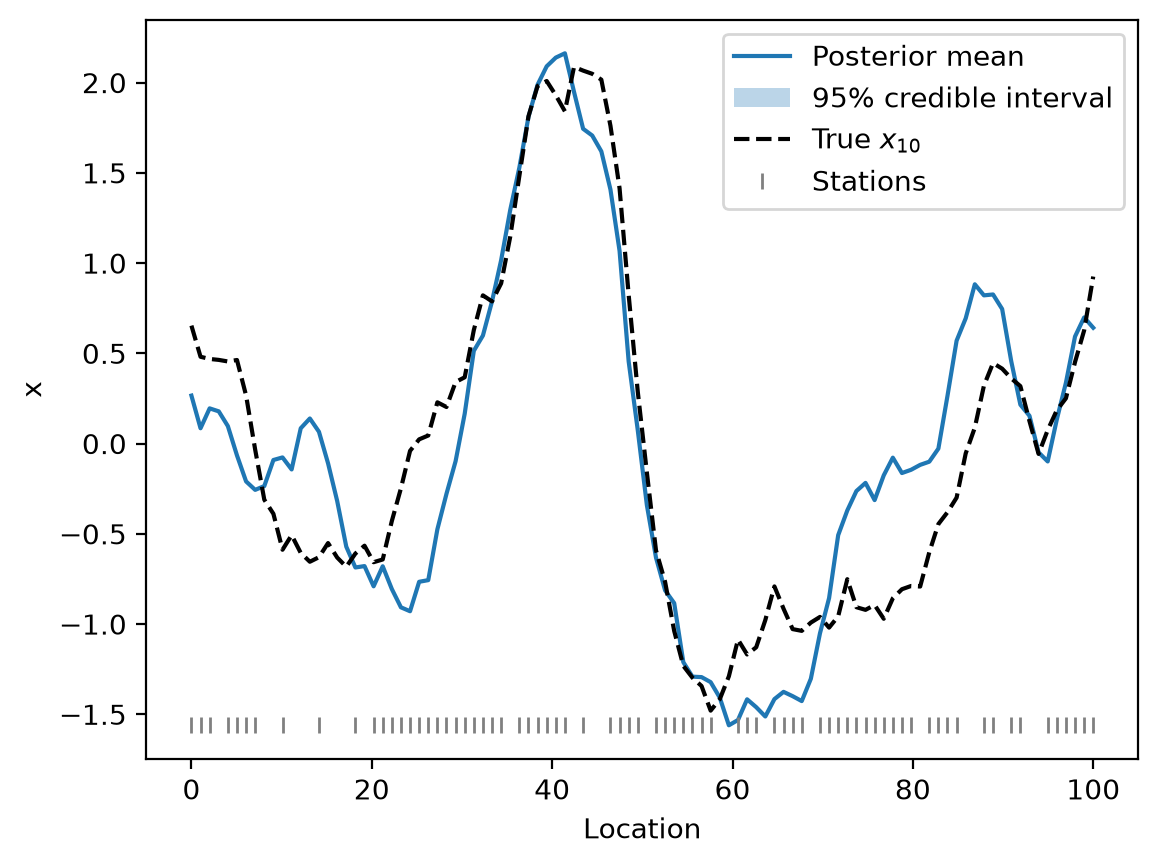
\includegraphics[width=\linewidth]{code/simulation/figures/particle_filter_filtering_band.png}
        \caption{Particle filter ($N = 1000$)}
    \end{subfigure}
    \hfill
    \begin{subfigure}{0.48\textwidth}
        \centering
        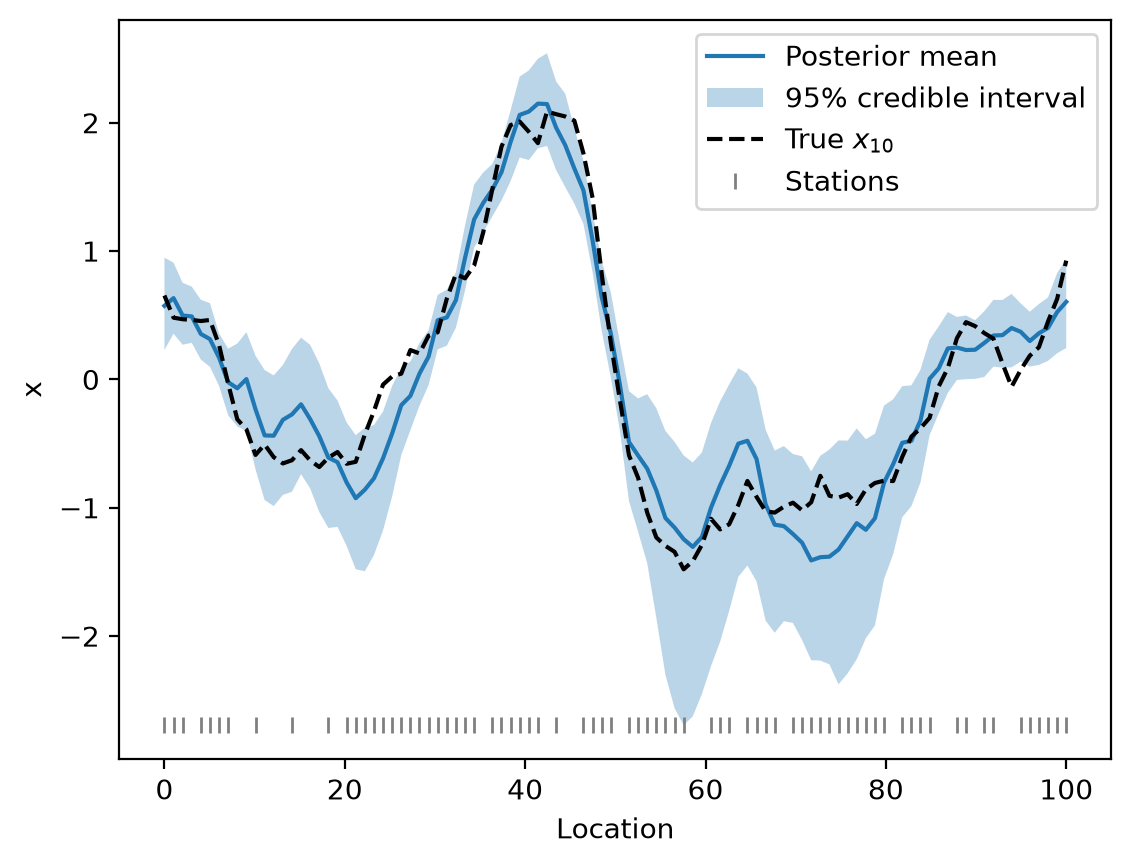
\includegraphics[width=\linewidth]{code/simulation/figures/penkf_filtering_band.png}
        \caption{PEnKF ($N = 100$ $\theta$ ensembles, $M = 10$ members per ensemble)}
    \end{subfigure}

    \vspace{1em}
    \begin{subfigure}{0.48\textwidth}
        \centering
        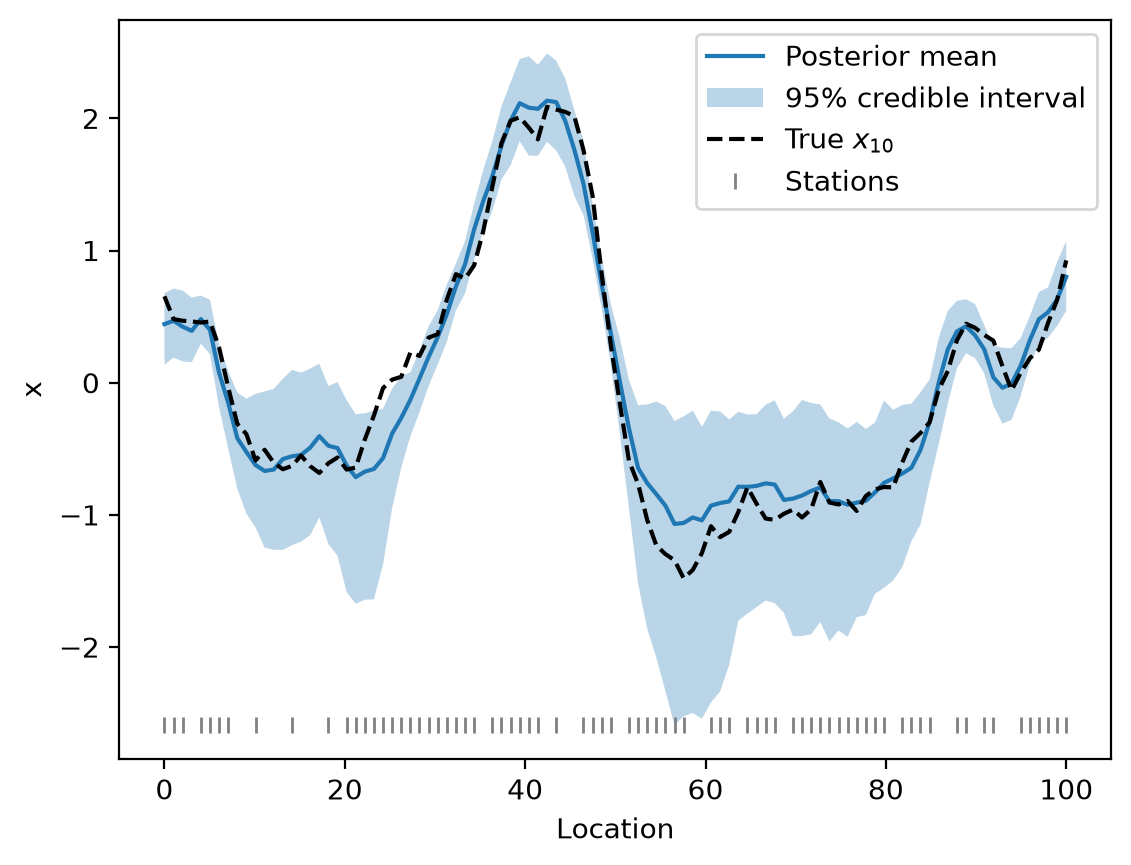
\includegraphics[width=\linewidth]{code/simulation/figures/genkf_filtering_band.png}
        \caption{GEnKF ($M = 100$ members)}
    \end{subfigure}
    \caption{Filtering distribution of $\vx_{10}$: posterior mean, 95\% credible
    band, and the true state, with the observing stations marked on the bottom.
    The particle filter and the PEnKF use systematic resampling. Due to 
    weight-degeneracy, the credible interval of the particle filter collapses.}
    \label{fig:filtering-bands}
\end{figure}

\begin{table}[ht]
    \centering
    \begin{tabular}{lcc}
        \toprule
        Method & RMSPE & CRPS \\
        \midrule
        Prior & 0.965 & 0.561 \\
        Particle filter & 0.420 & 0.341 \\
        PEnKF & 0.257 & 0.153 \\
        GEnKF & \textbf{0.184} & \textbf{0.120} \\
        \bottomrule
    \end{tabular}
    \caption{Accuracy of the filtering distribution of $\vx_{10}$. RMSPE is the
    root mean squared error of the posterior mean over the grid, and CRPS is
    averaged over the grid. The prior row draws states from the prior and
    ignores the observations. The best value in each column is in bold.}
    \label{tab:filtering-metrics}
\end{table}

% Both ensemble methods track the true state, and the true $\theta_{10}$ lies
% within the bulk of both distributions of $\theta$. Even with systematic resampling, the particle
% filter's weights collapse onto essentially a single particle at every step (an
% effective sample size of about $1$ out of $1000$), so its band is degenerate
% and its posterior mean is the least accurate of the three. The GEnKF has the
% lowest RMSPE and CRPS.

% Implementation

% Show plots of predictions, RMSPE, CRPS
% Conclusion, visually looks good, it can be done
% Note: this was difficult to derive, and possibly almost impossible if
% we don't have independence of thetas
% Limitation... lack of ground truth
% Other limitation... this was with linear AR-(1) model
% GEnKF was relatively slow to run even on this toy example due to nested
% quadrature, PEnKF was fast thanks to approximation, but if we had to 
% use quadrature it would have been super slow as well

\subsection{Weight-degeneracy}\label{sec:weight}
% Run PEnKF without resampling
% Weight degeneracy, show particle filter and ESS of PEnKF
% Conclusion - yes PEnKF somewhat solves the weight degeneracy, problem but
% it's far from perfect.
% Can do a 
The second question we wish to answer is whether the PEnKF empirically solves
the weight-degeneracy problem. To evaluate the severity of weight-degeneracy,
we use the importance sampling ESS for
normalized weights $w^1, \ldots, w^N$ \cite{kong1994,kong1992,chopin2020} defined by
\begin{align}
    \text{ESS} = \frac{1}{\sum_{i=1}^N (w^i)^2}.
\end{align}
On the same dataset, we run the particle filter and PEnKF with no resampling,
in addition to our previous runs with resampling.
Results are shown in Table~\ref{tab:ess}, and are clearly poor for the particle
filter -- an ESS of 1 indicates that practically all the weight is on a single
sample. This agrees with what we see in Figure~\ref{fig:filtering-bands}. The
ESS for the PEnKF is not great, but is still significantly better than the
particle filter. With frequent resampling, the PEnKF is still able to capture
the distribution of $\theta$ reasonably well, especially considering that
$\theta$ is 1-dimensional in our study. Fluctuations in the ESS for the PEnKF
may be due to unexpected observations; very unexpected observations cause large
shifts in the distribution which are difficult to capture by reweighting. We
conclude that the PEnKF does moderately well at addressing weight-degeneracy,
although it could be better.

\begin{table}[ht]
    \centering
    \small
    \begin{tabular}{lcccccccc}
        \toprule
        & \multicolumn{4}{c}{No resampling} & \multicolumn{4}{c}{Resampling} \\
        \cmidrule(lr){2-5} \cmidrule(lr){6-9}
        & \multicolumn{2}{c}{Particle filter} & \multicolumn{2}{c}{PEnKF}
        & \multicolumn{2}{c}{Particle filter} & \multicolumn{2}{c}{PEnKF} \\
        \cmidrule(lr){2-3} \cmidrule(lr){4-5} \cmidrule(lr){6-7} \cmidrule(lr){8-9}
        $t$ & ESS & ESS$/N$ & ESS & ESS$/N$ & ESS & ESS$/N$ & ESS & ESS$/N$ \\
        \midrule
        1 & 1.00 & 0.001 & 1.86 & 0.019 & 1.00 & 0.001 & 1.86 & 0.019 \\
        2 & 1.00 & 0.001 & 3.27 & 0.033 & 1.01 & 0.001 & 7.16 & 0.072 \\
        3 & 1.00 & 0.001 & 3.09 & 0.031 & 1.00 & 0.001 & 13.58 & 0.136 \\
        4 & 1.00 & 0.001 & 1.00 & 0.010 & 1.00 & 0.001 & 2.82 & 0.028 \\
        5 & 1.00 & 0.001 & 1.00 & 0.010 & 1.00 & 0.001 & 2.05 & 0.021 \\
        6 & 1.00 & 0.001 & 1.00 & 0.010 & 1.12 & 0.001 & 13.30 & 0.133 \\
        7 & 1.00 & 0.001 & 1.00 & 0.010 & 1.00 & 0.001 & 22.95 & 0.230 \\
        8 & 1.00 & 0.001 & 1.78 & 0.018 & 1.03 & 0.001 & 7.94 & 0.079 \\
        9 & 1.00 & 0.001 & 1.00 & 0.010 & 1.17 & 0.001 & 3.28 & 0.033 \\
        10 & 1.00 & 0.001 & 1.35 & 0.013 & 1.00 & 0.001 & 15.27 & 0.153 \\
        \bottomrule
    \end{tabular}
    \caption{ESS of the importance weights at each time
    step, and the ESS as a fraction of the number of particles $N$, computed
    before any resampling at that step. The particle filter uses $N = 1000$
    particles, and the PEnKF uses $N = 100$ particles with $M = 10$ ensemble
    members each. With resampling, the weights are reset to equal whenever the
    ESS falls below $0.66N$.}
    \label{tab:ess}
\end{table}

\subsection{Practicality of forecast independence}\label{sec:one_step}
% Does the state-space model actually help here or are time steps too
% different from one another?

% Future simulation studies could look at the generative process itself, here
% we look just at the predictive errors that show up from the one-ste
% prediction process.
Finally, we address the question of how restrictive the forecast independence
conditions are, particularly the requirement for independent $\theta_t$. To
probe this question, we propose the following hypothesis: if the $\theta_t$ are
independent, then a state-space model is not meaningfully more expressive than a
model which treats each time step independently. We test the following corollary
of the hypothesis: if the $\theta_t$ are independent, then an estimator which
sees past time points will not do significantly better than an estimator that
doesn't. To this end, we run a particle filter, GEnKF and PEnKF but only at time
$t=10$ without observations from $t=1, \ldots, 9$, and compare the performance
of the estimate of the latent state $\vx$ to that from a particle filter, GEnKF
and PEnKF which see observations from all ten time points.

Plots of the posterior 95\% credible intervals for each method are shown in 
Figure~\ref{fig:single-update-bands}. Again, we have significant
weight-degeneracy for the particle filter. Qualitatively, the particle filter and PEnKF
are much worse than their counterparts with access to the full dataset, although
the poor performance of the PEnKF and particle filter is partly explained by
weight-degeneracy and the significant distance between prior and posterior.  It
is harder to tell for the GEnKF, as both actually provide reasonable posterior
means. Nevertheless, the GEnKF shows a large quantitative penalty from only
seeing the last data point, as seen in Table~\ref{tab:single-update-metrics}. We
conclude that observations from previous time points have a noticeable impact on
inference in this model, and thus forecast independence is not necessarily a
completely destructive constraint.

\begin{figure}[htbp]
    \centering
    \begin{subfigure}{0.48\textwidth}
        \centering
        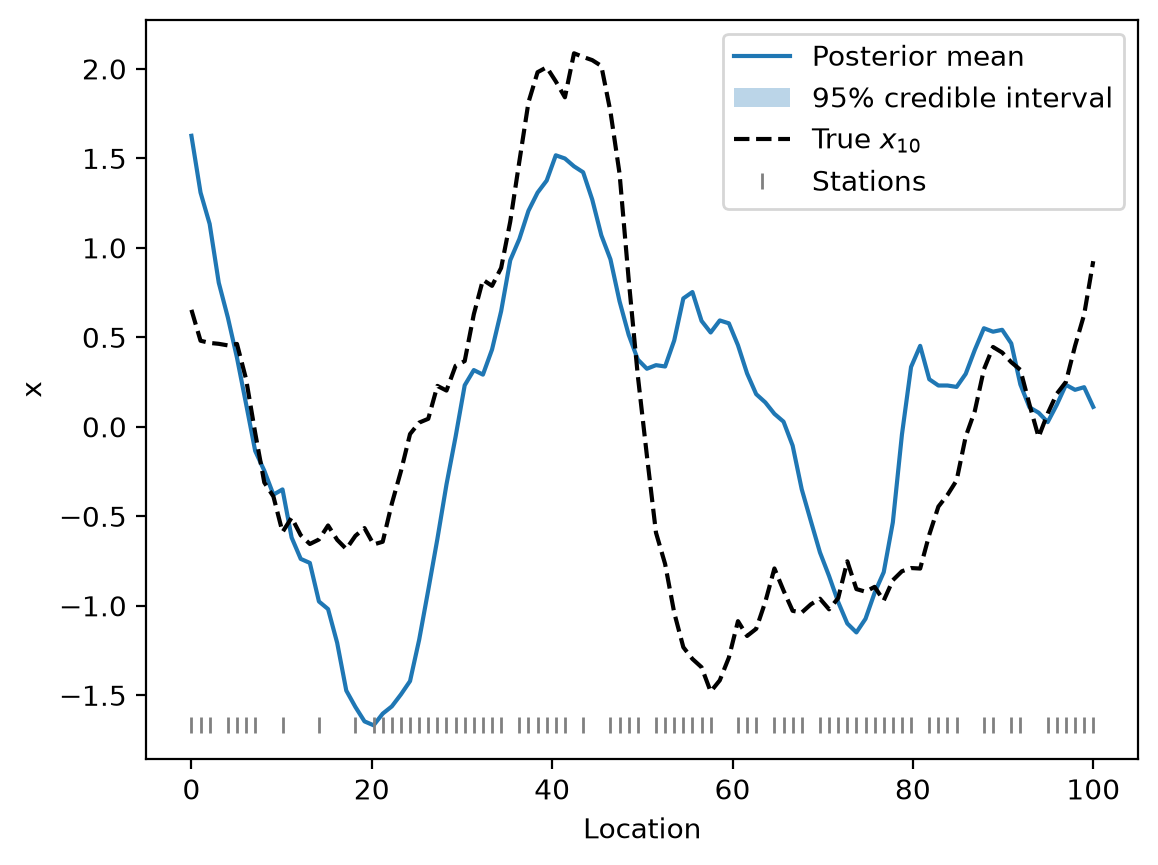
\includegraphics[width=\linewidth]{code/simulation/figures/particle_filter_single_update_band.png}
        \caption{Particle filter ($N = 1000$)}
    \end{subfigure}
    \hfill
    \begin{subfigure}{0.48\textwidth}
        \centering
        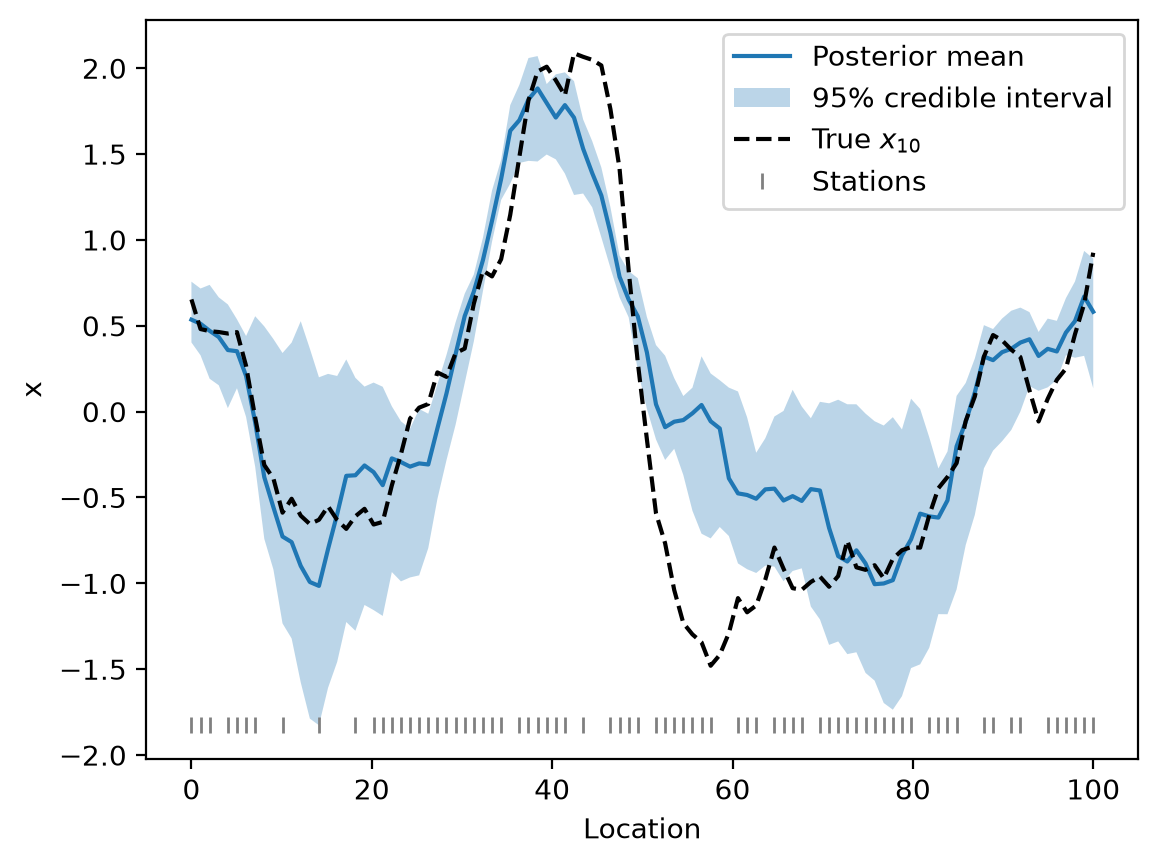
\includegraphics[width=\linewidth]{code/simulation/figures/penkf_single_update_band.png}
        \caption{PEnKF ($N = 100$ particles, $M = 10$ members)}
    \end{subfigure}

    \vspace{1em}
    \begin{subfigure}{0.48\textwidth}
        \centering
        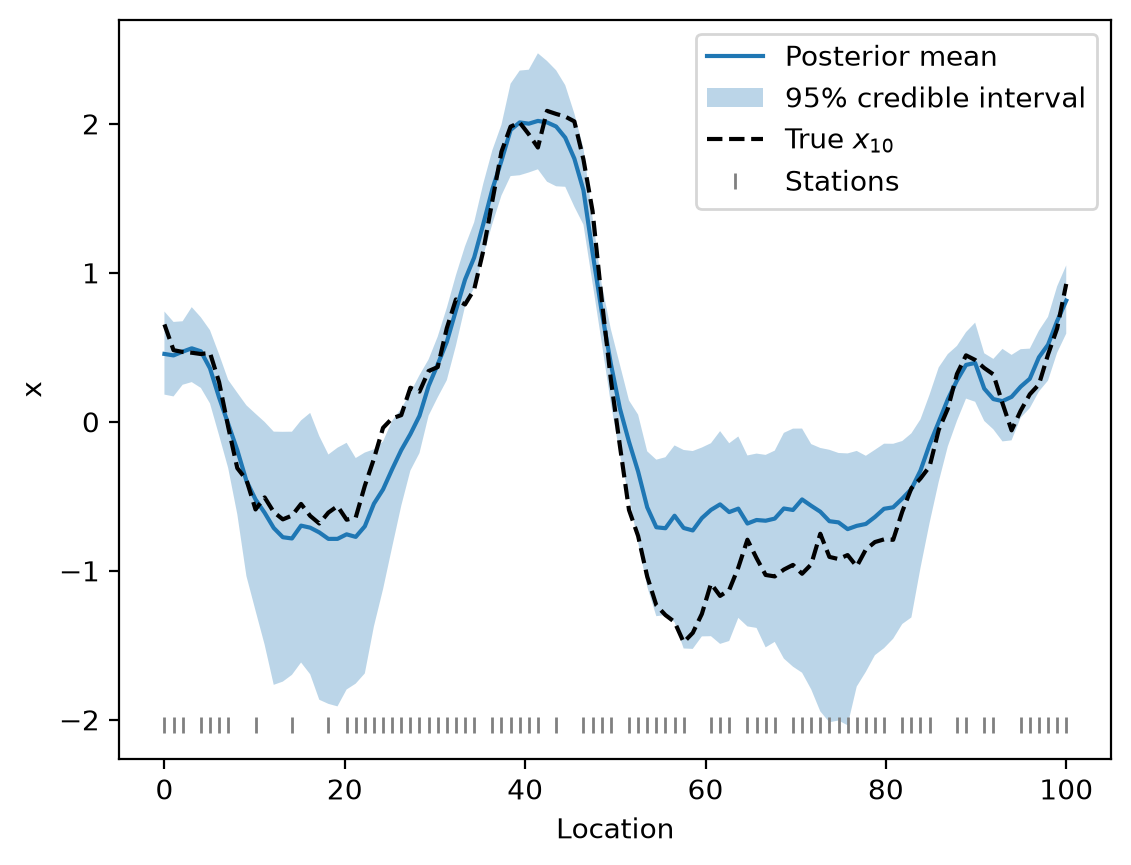
\includegraphics[width=\linewidth]{code/simulation/figures/genkf_single_update_band.png}
        \caption{GEnKF ($M = 100$ members)}
    \end{subfigure}
    \caption{Distribution of $\vx_{10}$ given only the observations at $t=10$:
    posterior mean, 95\% credible band, and the true state, with the observing
    stations marked on the bottom.}
    \label{fig:single-update-bands}
\end{figure}

\begin{table}[ht]
    \centering
    \begin{tabular}{lcccc}
        \toprule
        & \multicolumn{2}{c}{All ten time points} & \multicolumn{2}{c}{Final time point only} \\
        \cmidrule(lr){2-3} \cmidrule(lr){4-5}
        Method & RMSPE & CRPS & RMSPE & CRPS \\
        \midrule
        Particle filter & 0.420 & 0.341 & 0.821 & 0.634 \\
        PEnKF & 0.257 & 0.153 & 0.446 & 0.269 \\
        GEnKF & \textbf{0.184} & \textbf{0.120} & \textbf{0.271} & \textbf{0.154} \\
        \bottomrule
    \end{tabular}
    \caption{Accuracy of the distribution of $\vx_{10}$ when each method sees
    all ten time points or only the final one. RMSPE is the root mean squared
    error of the posterior mean over the grid, and CRPS is averaged over the
    grid. The best RMSPE and CRPS in each column is in bold.}
    \label{tab:single-update-metrics}
\end{table}

\subsection{Repeated seeds}
We repeat the experiments in Sections~\ref{sec:full}, \ref{sec:weight} and
\ref{sec:one_step} across 30 different seeds in a full simulation study.
Table~\ref{tab:replicates} reports the mean accuracy of each method over $30$
simulated datasets, and the paired differences between methods within each
dataset. These results confirm that the GEnKF performs significantly better
than the PEnKF, which in turn performs significantly better than the particle
filter on its own. The ESS values of the particle filter and the
PEnKF over these datasets are reported in Appendix~\ref{sec:ess_replicates},
and agree with our single-seed experiment from the previous sections.

\begin{table}[tbp]
    \centering
    \small
    \renewcommand{\arraystretch}{1.25}
    \begin{tabular}{lcccc}
        \toprule
        & \multicolumn{2}{c}{All ten time points} & \multicolumn{2}{c}{Final time point only} \\
        \cmidrule(lr){2-3} \cmidrule(lr){4-5}
        & RMSPE & CRPS & RMSPE & CRPS \\
        \midrule
        \multicolumn{5}{l}{\emph{Mean over datasets [95\% confidence interval]}} \\
        \shortstack[l]{Prior \\ {\scriptsize\phantom{[0]}}} & \shortstack{0.955 \\ {\scriptsize [0.867, 1.044]}} & \shortstack{0.551 \\ {\scriptsize [0.500, 0.601]}} & \shortstack{0.955 \\ {\scriptsize [0.867, 1.044]}} & \shortstack{0.551 \\ {\scriptsize [0.500, 0.601]}} \\
        \shortstack[l]{Particle filter \\ {\scriptsize\phantom{[0]}}} & \shortstack{0.562 \\ {\scriptsize [0.517, 0.608]}} & \shortstack{0.427 \\ {\scriptsize [0.392, 0.462]}} & \shortstack{0.686 \\ {\scriptsize [0.611, 0.760]}} & \shortstack{0.538 \\ {\scriptsize [0.486, 0.589]}} \\
        \shortstack[l]{PEnKF \\ {\scriptsize\phantom{[0]}}} & \shortstack{0.411 \\ {\scriptsize [0.367, 0.454]}} & \shortstack{0.227 \\ {\scriptsize [0.204, 0.249]}} & \shortstack{0.529 \\ {\scriptsize [0.464, 0.594]}} & \shortstack{0.323 \\ {\scriptsize [0.283, 0.364]}} \\
        \shortstack[l]{GEnKF \\ {\scriptsize\phantom{[0]}}} & \shortstack{\textbf{0.341} \\ {\scriptsize [0.285, 0.397]}} & \shortstack{\textbf{0.170} \\ {\scriptsize [0.145, 0.195]}} & \shortstack{\textbf{0.384} \\ {\scriptsize [0.319, 0.449]}} & \shortstack{\textbf{0.193} \\ {\scriptsize [0.162, 0.224]}} \\
        \midrule
        \multicolumn{5}{l}{\emph{Paired difference between methods [95\% confidence interval]}} \\
        \shortstack[l]{GEnKF $-$ PEnKF \\ {\scriptsize\phantom{[0]}}} & \shortstack{$-0.069$ \\ {\scriptsize [$-0.105$, $-0.033$]}} & \shortstack{$-0.057$ \\ {\scriptsize [$-0.079$, $-0.035$]}} & \shortstack{$-0.145$ \\ {\scriptsize [$-0.180$, $-0.110$]}} & \shortstack{$-0.130$ \\ {\scriptsize [$-0.157$, $-0.104$]}} \\
        \shortstack[l]{GEnKF $-$ Particle filter \\ {\scriptsize\phantom{[0]}}} & \shortstack{$-0.221$ \\ {\scriptsize [$-0.269$, $-0.173$]}} & \shortstack{$-0.257$ \\ {\scriptsize [$-0.289$, $-0.225$]}} & \shortstack{$-0.301$ \\ {\scriptsize [$-0.357$, $-0.246$]}} & \shortstack{$-0.345$ \\ {\scriptsize [$-0.384$, $-0.306$]}} \\
        \shortstack[l]{PEnKF $-$ Particle filter \\ {\scriptsize\phantom{[0]}}} & \shortstack{$-0.152$ \\ {\scriptsize [$-0.189$, $-0.114$]}} & \shortstack{$-0.200$ \\ {\scriptsize [$-0.227$, $-0.174$]}} & \shortstack{$-0.156$ \\ {\scriptsize [$-0.220$, $-0.092$]}} & \shortstack{$-0.214$ \\ {\scriptsize [$-0.267$, $-0.162$]}} \\
        \bottomrule
    \end{tabular}
    \caption{Accuracy of the distribution of $\vx_{10}$ over 30 simulated datasets,
    when each method sees all ten time points or only the final one. RMSPE is the
    root mean squared error of the posterior mean over the grid, and CRPS is
    averaged over the grid. Each entry is a mean over datasets, with its 95\%
    confidence interval in brackets below, using the $0.975$ quantile of the $t$
    distribution with 29 degrees of freedom. The best mean in each column is in
    bold. The prior ignores the observations, so it is the same in both column
    groups. The paired differences are taken within each dataset, where all
    methods see the same data, and a negative value means that the first method
    has the smaller error.}
    \label{tab:replicates}
\end{table}



% Also... if time, compare directly to running HMC with that target.

\section{Discussion}


% In the rainfall simulation we are currently using a linear model, with Gaussian
% prior on the latent state $x$. In such a case, the EnKF update is asymptotically
% exact \cite{evensen2009}, and so a very high particle versin of the GEnKF could
% serve as the ground truth.

While this qualifying paper expands the experimental coverage of the GEnKF and
PEnKF inference methods, our experiments are by no means exhaustive. One big
limitation is our lack of a complete picture of ``ground truth''. While we know
the latent state used by the true data generating process, we would ideally be
able to compare the GEnKF and the PEnKF to a sample from the true filtering
distribution, as both the GEnKF and PEnKF introduce approximations. A very large
particle PEnKF with a large quadrature approximation of the PEnKF likelihood
could be used for such a ground truth.  Furthermore, in our existing experiments
we note that the GEnKF took significantly longer to run (on the order of
minutes) compared to the particle filter and PEnKF (order of seconds). We have
already accounted for this difference to some degree by using only tracking
$100$ latent-states in the GEnKF, as opposed to $1000$ total latent states for
the particle filter and PEnKF. However, future experiments could measure and
control for this difference more rigorously.  In particular, it would also be
useful to consider using quadrature for the PEnKF likelihood, which would take
longer, but give more accurate weights. Another experimental condition that we
may consider changing is breaking the linear dynamics.  Under linear dynamics,
the EnKF is asymptotically exact. This translates to asymptotic exactness of the
PEnKF update, as each update is performed on a Gaussian ensemble (although we
lose this exactness if we use an approximation of the likelihood).  However, it
does not translate to asymptotic exactness of the GEnKF, because its EnKF update
is performed on a mixture of normals.  Nevertheless, we hypothesize that under
highly non-linear dynamics both the GEnKF and PEnKF will perform significantly
worse. The final experimental limitation we note is the inability of our single
time step experiment to distinguish inadequacy of the inference method from
inadequacy of the model. This could be improved by using more particles and
longer compute times to overcome inadequacies in inference.

% Proposed extensions

One potential methodological extension is to use the analytic form of the
Kalman filter for the PEnKF when dynamics are linear. While this would require
carrying a dense covariance matrix instead of a particle ensemble, there may
be a sweet spot in moderate dimensions where this method has less variability
than ensemble methods, but dimensionality is not too high to make instantiating
this matrix infeasible. Such a method would not work naively for the GEnKF,
because in the GEnKF the EnKF update is applied over the marginal distribution
of $\vx$, which is no longer normal, whereas in the PEnKF it is applied to the
conditional distribution, which is normal.

Another relatively simple extension to the existing methodology is to use
the EnKF update as a proposal distribution for the state update in an SMC filter.
This method would allow for asymptotic consistency as the number of particles
goes to infinity, while still addressing the weight-degeneracy evident in the
bootstrap particle filter. An outline of this proposed algorithm is given below:
\begin{enumerate}
    \item Sample $(\theta^i_0, \vx^i_0)$ from the prior
    \item For $t=1,\ldots,T$
    \begin{enumerate}
        \item For each particle $i$
        \begin{enumerate}
            \item Draw a new proposal $\theta^i_t$ from $p(\theta_t \mid \theta^i_{t-1})$
            \item Propagate each element of the ensemble under
            the model; $\tilde \vx^i_t = \mathcal M(\vx^i_{t-1}; \theta^i_t)$
        \end{enumerate}
        \item Estimate the mean and covariance of the forecast distribution using
        the entire ensemble
        \item Compute a global EnKF gain matrix $\mathbf K$ based on the estimates from
        the entire ensemble
        \item For each particle
        \begin{enumerate}
            \item Propose $\vx^i_t \sim q(\vx^i_t) = \Norm_d(\boldsymbol\mu^i, \mathbf\Sigma^i)$, where
            \begin{align}
                \boldsymbol\mu^i &= \tilde\vx^i_t + \mathbf K(\vy - \mathbf H\tilde\vx^i_t) \\
                \mathbf\Sigma^i &= \mathbf Q + \mathbf K\mathbf R\mathbf K^\top,
            \end{align}
            and $\vy$ refers to the noiseless observation
            \item Update weights according to 
            \begin{align}
                w^i_t &= w^i_{t-1}\mathcal L(\theta^i_t, \vx^i_t; \vz_t)\frac{p(\vx^i_t)}{q(\vx^i_t)},
            \end{align}
            where $p(\vx^i_t) = \Norm_d(\vx^i_t; \tilde \vx^i_t, \mathbf Q)$ is the density
            of the bootstrap proposal based solely on model dynamics
        \end{enumerate}
    \end{enumerate}
\end{enumerate}
One potential weakness of this method is that the marginal uncertainty of $\vx$
will typically overstate the uncertainty conditional on $\theta_t^i$
(which is what we would ideally use). This could be combatted by using locally
weighted estimates of the covariance based on points with similar $\theta$
values. In the case of forecast independence, the conditional and marginal
covariances are identical, and this proposed algorithm may perform well. In such
cases, we conjecture that it may also be significantly faster than the GEnKF.

% We also propose one simple methodological extension that appears to have been
% missed by the original authors. When the dynamics are linear, the Kalman filter
% is actually exact. Thus instead of using an EnKF update in the PEnKF, we can
% simply use the anlaytic Kalman filter update, and instead of keeping track of
% ensemble.......

% The key point of the EnKF is that it approximates a transport map from 
% prior to posterior, by using that which we would use for Gaussian. We could 
% attempt to define a stochastic transport map for any such conjugate family  
% Could really use any conditionally conjugate family

% Limitations of our experiments
% Only a single simulation... could repeat with different dataset and seeds
% to get a full picture of how well these methods perform in this scenario
% Lack of ground truth even in relatively simple scenario
% Have not analyzed s

% Improvements could be made by tuning... this would be tedious but would
% provide the fairest comparison

% Future experiments
% - standardize compute budget
% - break linearity
% - larger simulation study

\section{Conclusion}
In this qualifying paper we provide a critique and empirical investigation of the
GEnKF and PEnKF that were proposed in \cite{katzfuss2020}. These two methods combine
SMC with the EnKF to tackle state-space models with
both high-dimensional latent variables and parameters that are not well
described by normality assumptions. Our main methodological critiques focus on
the restrictiveness of the assumptions required to implement the GEnKF, and the
difficulty of the nested sampling or quadrature required to implement both
methods. Furthermore, the numerical experiments in the original paper
\cite{katzfuss2020} leave many basic questions unanswered. Most importantly,
there is no experimental analysis of the GEnKF with a separate parameter layer,
no head-to-head comparison of GEnKF and PEnKF on the same model, no analysis
of GEnKF in a model with more than one time step, and limited experimental
discussion of the weight-degeneracy problem.

We explore these experimental gaps using a simulation study that extends the
rainfall model used in \cite{katzfuss2020}.  Our experimental results are
relatively positive for the GEnKF and the PEnKF.  Indeed, we find that both
perform much better in terms of RMSPE and CRPS than the particle filter, which
suffers from severe weight-degeneracy. The GEnKF also performs better than the
PEnKF. However, further work is needed to identify whether this is because of
approximations used in the PEnKF likelihood, the tuning parameters chosen, or an
inherent relative weakness in the PEnKF method. Additionally, the importance
sampling ESS was used to quantitatively analyze the weight-degeneracy problem in
the PEnKF. While the PEnKF maintained a non-negligible relative ESS, 
resampling was required at almost every step to prevent significant
degeneration. Lastly, we investigate whether the forecast independence conditions
are overly restrictive on the state-space model. We find that restricting the
GEnKF and PEnKF to only the last time step reduces their performance. This
provides evidence, though not proof, that the class of state-space models
with forecast independence is meaningfully more expressive than completely
assuming temporal independence, although we maintain that it is still highly
restrictive. Future work may focus on treating the EnKF update as a proposal
within an SMC framework, as opposed to an exact update. This will allow for
asymptotic exactness which is not available to the GEnKF and the PEnKF under
non-linear model dynamics.

\section{Statement on the use of large language models (LLMs)}
LLMs were used for the following:
\begin{itemize}
    \item Assistance with coding, particularly generating graphs, input and output
    operations, refactoring, transpiling R to Python, and HMC code
    \item Typesetting: formatting graphs, figures and tables. Creating TikZ
    figures
    \item Assistance with managing references and BibTeX entries
    \item Reviewing spelling and grammar
    \item Reviewing mathematical proofs and notational consistency
\end{itemize}

% Planning notes
% Not really using ensemble Kalman updates? N \times M issue

% Background Kalman filter Extended Kalman Filter Ensemble Kalman Filter
% Particle filter methods

% This methodology
% GenKF
% PenKF

% Computer experiments
% Implemenet the GenKF and PenKF
% Reproduce the results from the paper
% If time
%  - Check robustness to different priors, non-linear dynamics. Compare to particle filters

% Discussion
% Critical analysis of this method
%   Strengths
%   - Fast (low rank, sample)
%   - Flexible (handles hierarhical models and parametesr not handled well by state augemtnation)
%   Weaknesses
%   - Sacrifices asymptotic correctness
% Propsal extension methods
%   - What if we try to learn a flow or an SDE instead of using Kalmn filter updates?
%   - If time work out the math here

\bibliographystyle{unsrt}
\bibliography{refs}

\clearpage % flush the figures and tables of the main text
\appendix
\section{Rainfall model}\label{sec:rainfall_appendix}
Throughout this section we drop subscripts related to time for ease of reading.
All distributions are assumed to be conditional on $\vz_{1:t-1}$, even if this
is not stated in the notation.

\subsection{Particle filter likelihood}\label{sec:pf_likelihood}
For the particle filter we require the log-likelihood.
\begin{align}
    \mathcal L(\theta, \vx; \vz)
\end{align}
The particle filter tracks $\vx$ and $\theta$, so we use the conditional log-likelihood
marginalizing over $\vy$. We have a point mass at zero, so instead of considering
densities with respect to the Lebesgue measure, we consider densities with
respect to the Lebesgue measure plus a Dirac delta at zero. Letting
$m$ be the dimension of $\vy$, $\lambda$ the Lebesgue measure and $\delta_0$
the Dirac delta measure at $0$, we are using the likelihood with respect to
\begin{align}
    \nu := (\lambda + \delta_0)^{\otimes m}
\end{align}
Given the model in 
Example~\ref{ex:rainfall}, the coordinates $y_l$ of $\vy$ are independent conditional
on $\vx$. This simplifies the likelihood. Based on the Jacobian of the
transformation from $\vy$ to $\vz$, we can find the likelihood as a product
over observation locations
\begin{align}
    \mathcal L(\theta, \vx; \vz) &:= 
        \prod_l \mathcal L_l(\theta, x_l; z_l) \\
    \mathcal L_l(\theta, x_l; z_l) &:=
        \begin{cases}
            \Phi\left(-\frac{x_l}{\sigma_t}\right)\quad &\text{if } z_l = 0 \\
            \frac{1}{\theta\sigma_t}z_l^{\frac 1 \theta - 1}\Norm\left(\frac{z_l^{1/\theta}-x_l}{\sigma_t}; 0, 1\right)\quad &\text{else}
        \end{cases},
\end{align}
where $l$ ranges over observation locations and $\Phi$ is the standard normal cumulative distribution function. The $z > 0$ term agrees with that
presented in \cite{katzfuss2020}. They omit the $z=0$ term, because they
presented the likelihood in the context of the GEnKF, which does not use the
log-likelihood for updates of $x$. However, to use this for the particle filter,
we must include this term.

\subsection{PEnKF likelihood}\label{sec:penkf_likelihood}
For the PEnKF we need the marginal likelihood
\begin{align}
    \mathcal L(\theta; \vz)
\end{align}
In essence we must marginalize the particle filter likelihood over $\vx$. In
general, \cite{katzfuss2020} suggest using an approximation of the likelihood
based on the EnKF. Given a $\theta^i$, their procedure is as follows
\begin{enumerate}
    \item Propagate the ensemble to get $\tilde\vx_t^{ij} = \mathcal M(\vx_{t-1}^{ij};\theta^i_t)$
    \item Estimate $\boldsymbol\mu$ and $\tilde{\mathbf\Sigma}$, the mean and covariance of the propagated
    ensemble
    \item Approximate the ``prior'' on $\vx_t$ by a normal with mean $\boldsymbol\mu$ and
    covariance $\widehat{\mathbf\Sigma} = \tilde{\mathbf\Sigma} + \mathbf Q$ 
    \item Calculate the integral (by quadrature if necessary)
    \begin{align}
        p(\vz_t \mid \theta_{1:t}, \vz_{1:t-1}) &=
            \int p(\vz_t \mid \vy_t, \theta_t)\Norm_{m_t}(\vy_t;\mathbf H\boldsymbol\mu,\mathbf H\widehat{\mathbf\Sigma}\mathbf H^\top + \mathbf R)\,d\vy_t \label{eq:enkf_likelihood}
    \end{align}
\end{enumerate}
In our case, the observation model is conditionally deterministic given
$\vy_t$ and $\theta_t$. Due to the changing support, this would make
Equation~\eqref{eq:enkf_likelihood} unwieldy. We work directly with the
likelihood presented in Section~\ref{sec:pf_likelihood}.
\begin{align}
    \mathcal L(\theta, \vx; \vz) &=
        \begin{cases}
            \Phi\left(-\frac{x_l}{\sigma_t}\right)\quad &\text{if } z_l = 0 \\
            \frac{1}{\theta\sigma_t}z_l^{\frac 1 \theta - 1}\Norm\left(\frac{z_l^{1/\theta}-x_l}{\sigma_t}; 0, 1\right)\quad &\text{else}
        \end{cases}
\end{align}
as before with respect to the mixed measure $(\lambda + \delta_0)^{\otimes m}$.
To find $\mathcal L(\theta; \vz)$ we marginalize over $\vx$
\begin{align}
   \mathcal L(\theta; \vz) &= \int p(\vz \mid \vx,\theta)p(\vx \mid \theta)\,d\vx
\end{align}
The conditional distribution $p(\vx \mid \theta)$ is approximated by adding noise to
the forecasting distribution to get $p(\vx \mid \theta) = \Norm_d(\vx; \boldsymbol\mu, \tilde{\mathbf\Sigma} + \mathbf Q)$. Using the independence assumption
\begin{align}
    \int p(\vz \mid \vx,\theta)p(\vx \mid \theta)\,d\vx 
    &= \int \prod_l p(z_l \mid x_l, \theta)p(\vx \mid \theta)\,d\vx \label{eq:penkf_integral}
\end{align}

\subsection{A diagonal approximation}

We can analytically solve the integral in Equation~\eqref{eq:penkf_integral} in
the case of a diagonal approximation to $\tilde{\mathbf\Sigma} + \mathbf Q$. We make
use of two lemmas.

\begin{lemma}\label{lemma:icdf}
    If $X \sim \Norm(\mu, \sigma^2)$ then
    $\E\Phi(X) = \Phi\left(\frac{\mu}{\sqrt{1+\sigma^2}}\right)$
\end{lemma}
\begin{proof}
    From the definition of the cumulative distribution function and the tower rule
    \begin{align}
        \Phi(X) &= \P(Z \leq X \mid X) \quad Z \sim \Norm(0,1) \perp X \\
        \E\Phi(X) &= \P(Z \leq X) \\
        &= \P(Z - X \leq 0)
    \end{align}
    But since $X$ and $Z$ are both normal and $X \perp Z$
    \begin{align}
        Z - X &\sim \Norm\left(-\mu, 1+\sigma^2\right) \\
        \P(Z-X \leq 0) &= \Phi\left(\frac{\mu}{\sqrt{1+\sigma^2}}\right)
    \end{align}
\end{proof}

\begin{lemma}\label{lemma:exponent}
    For $X \sim \Norm(\mu, \sigma^2)$
    \begin{align}
        \E\left[\frac{1}{\sqrt{2\pi}}\exp\left(-\frac{X^2}{2}\right)\right] &= 
            \frac{1}{\sqrt{2\pi(1+\sigma^2)}}\exp\left(-\frac{\mu^2}{2(1+\sigma^2)}\right)
    \end{align}
\end{lemma}
\begin{proof}
    We perform the integral by completing the square
    \begin{align}
        \E\left[\frac{1}{\sqrt{2\pi}}\exp\left(-\frac{X^2}{2}\right)\right] &= 
                \frac{1}{2\pi\sigma}\int \exp\left(-\frac{x^2}{2}\right)\exp\left(-\frac {1}{2\sigma^2}(x-\mu)^2\right) dx \\
        &= \frac{1}{2\pi\sigma}\int \exp\left(-\frac{x^2}{2}\right)\exp\left(-\frac{1}{2\sigma^2} \left(x^2 - 2x\mu + \mu^2 \right)\right) dx \\
        &= \frac{1}{2\pi\sigma}\int \exp\left(-\frac{1}{2\sigma^2}\left(x^2(1+\sigma^2) - 2x\mu + \mu^2 \right)\right) dx \\
        &= \frac{1}{2\pi\sigma}\int \exp\left(-\frac{1}{2\sigma^2}\left(x^2(1+\sigma^2) - 2x\mu + \frac{\mu^2}{1+\sigma^2} -  \frac{\mu^2}{1+\sigma^2} + \mu^2 \right)\right) dx\\
        &= \frac{1}{2\pi\sigma}\int \exp\left(-\frac{1}{2\sigma^2}\left((1+\sigma^2)\left(x - \frac{\mu}{1+\sigma^2}\right)^2 + \frac{\sigma^2\mu^2}{1+\sigma^2} \right)\right) dx\\
        &= \frac{1}{2\pi\sigma}\exp\left(-\frac 1 2\frac{\mu^2}{1+\sigma^2}\right)\int \exp\left(-\frac {1+\sigma^2}{2\sigma^2}\left(x - \frac{\mu}{1+\sigma^2}\right)^2\right) dx \\
        &= \frac{1}{2\pi\sigma}\exp\left(-\frac 1 2\frac{\mu^2}{1+\sigma^2}\right)\sqrt{\frac{2\pi\sigma^2}{1+\sigma^2}} \\
        &= \frac{1}{\sqrt{2\pi(1+\sigma^2)}}\exp\left(-\frac 1 2\frac{\mu^2}{1+\sigma^2}\right)
    \end{align}
    where the remaining integral is an unnormalized Gaussian integral, with $\int \exp\left(-\frac{a}{2}(x-m)^2\right)dx = \sqrt{2\pi/a}$ for $a = \frac{1+\sigma^2}{\sigma^2}$.
\end{proof}

Using the diagonal assumption, we simplify Equation~\eqref{eq:penkf_integral}
\begin{align}
    \int \prod_l p(z_l \mid x_l, \theta)p(\vx \mid \theta)\,d\vx &= 
    \prod_l \int p(z_l \mid x_l,\theta)p(x_l \mid \theta)\,dx_l
\end{align}
In the case $z_l=0$ with $x_l \sim \Norm(\mu_l, s^2_l)$, where $s^2_l$ is the $l$th diagonal entry of $\tilde{\mathbf\Sigma} + \mathbf Q$, we have
$\frac{-x_l}{\sigma_t} \sim \Norm\left(-\frac{\mu_l}{\sigma_t},\frac{s_l^2}{\sigma_t^2}\right)$, and by 
Lemma~\ref{lemma:icdf}
\begin{align}
    \E\left[p(z_l=0 \mid \theta, x_l) \mid \theta\right] &= \Phi\left(\frac{-\mu_l}{\sqrt{\sigma_t^2+s_l^2}}\right)
\end{align}
In the case $z > 0$, we note that
\begin{align}
    \frac{z_l^{\frac 1 \theta} - x_l}{\sigma_t} 
        \sim \Norm\left(\frac{z_l^{\frac 1 \theta} - \mu_l}{\sigma_t}, \frac{s_l^2}{\sigma_t^2}\right)
\end{align}
and so from Lemma~\ref{lemma:exponent}
\begin{align}
    \E p(z_l \mid \theta, x_l)
    &= \frac{1}{\theta\sigma_t}z_l^{\frac 1 \theta - 1}
        \E\left[\frac{1}{\sqrt{2\pi}}\exp\left(-\frac 1 2 \left(\frac{z_l^{1/\theta}-x_l}{\sigma_t}\right)^2\right)\right] \\
    &= \frac{1}{\theta\sigma_t}z_l^{\frac 1 \theta - 1}
        \frac{1}{\sqrt{2\pi\left(1+\frac{s_l^2}{\sigma_t^2}\right)}}
        \exp\left(-\frac{\left(z_l^{1/\theta}-\mu_l\right)^2}{2\left(\sigma_t^2+s_l^2\right)}\right) \\
    &= \frac{1}{\theta}z_l^{\frac 1 \theta - 1}\Norm\left(z_l^{1/\theta};\mu_l,\sigma_t^2+s_l^2\right)
\end{align}
We can also recognize this as the conditional probability $p(y_l \mid z_l,\theta)$ adjusted by the
Jacobian determinant $\frac{1}{\theta}z_l^{\frac{1}{\theta}-1}$.

% The independence assumption implies only the diagional elements of the
% covariance actually matter. 
% With deterministic trasnform, penkf jsut requires density estimator



\subsection{GEnKF - Metropolis within Gibbs}\label{sec:genkf_mcmc}
To implement the GEnKF we need to sample from the FCD of $\theta$ given by
\begin{align}
    p(\theta \mid \vx, \vy, \vz) \propto 
        p(\theta)p(\vx \mid \theta)p(\vy \mid \vx, \theta)p(\vz \mid \vy, \vx, \theta)
\end{align}
In the rainfall model, $p(\vy \mid \vx,\theta)$ does not depend on $\theta$, so this
simplifies to
\begin{align}
    p(\theta)p(\vx)p(\vy \mid \vx)p(\vz \mid \vy, \vx, \theta)
\end{align}
For $z=0$, $p(\vz \mid \vy, \vx, \theta)$ does not depend on $\theta$, which
further simplifies the likelihood. Up to a constant, the likelihood is
\begin{align}
    \mathcal L(\theta;\vx,\vy) := 
        p(\theta)\prod_{l:z_l > 0} \frac{1}{\theta}z_l^{\frac 1 \theta - 1}\Norm(z_l^{\frac 1 \theta};x_l,\sigma_t^2)
\end{align}
This agrees with what is presented in \cite{katzfuss2020}. The log-likelihood
up to a constant is then
\begin{align}
    \ell(\theta;\vx,\vy) := 
        \log p(\theta) + 
        \sum_{l:z_l > 0}\left[-\log \theta +\left(\frac 1 \theta - 1\right)\log z_l -\frac 1 {2\sigma_t^2}\left(z_l^{\frac 1 \theta}-x_l\right)^2\right]
\end{align}
with gradient
\begin{align}
    \nabla_\theta \ell(\theta;\vx,\vy) =
        \nabla_\theta \log p(\theta) +
        \sum_{l:z_l > 0}\left[-\frac 1 \theta - \frac{\log z_l}{\theta^2}
            + \frac{\log z_l}{\sigma_t^2\theta^2}z_l^{\frac 1 \theta}\left(z_l^{\frac 1 \theta}-x_l\right)\right]
\end{align}
In the rainfall model $\theta - 1 \sim \text{Gamma}(20, 10)$ (shape and rate),
so for $\theta > 1$
\begin{align}
    \log p(\theta) &= 20\log 10 - \log\Gamma(20) + 19\log(\theta - 1) - 10(\theta - 1) \\
    \nabla_\theta \log p(\theta) &= \frac{19}{\theta - 1} - 10
\end{align}

\section{ESS over repeated seeds}\label{sec:ess_replicates}
Table~\ref{tab:replicates-ess} reports the ESS of the importance
weights for the particle filter and the PEnKF over the same $30$ datasets as
Table~\ref{tab:replicates}.

\begin{table}[tbp]
    \centering
    \small
    \renewcommand{\arraystretch}{1.25}
    \begin{tabular}{lcccc}
        \toprule
        & \multicolumn{2}{c}{No resampling} & \multicolumn{2}{c}{Resampling} \\
        \cmidrule(lr){2-3} \cmidrule(lr){4-5}
        $t$ & Particle filter & PEnKF & Particle filter & PEnKF \\
        \midrule
        \shortstack[l]{1 \\ {\scriptsize\phantom{[0]}}} & \shortstack{1.02 \\ {\scriptsize [0.99, 1.05]}} & \shortstack{2.18 \\ {\scriptsize [1.61, 2.75]}} & \shortstack{1.06 \\ {\scriptsize [0.99, 1.14]}} & \shortstack{2.36 \\ {\scriptsize [1.86, 2.86]}} \\
        \shortstack[l]{2 \\ {\scriptsize\phantom{[0]}}} & \shortstack{1.05 \\ {\scriptsize [0.98, 1.13]}} & \shortstack{1.60 \\ {\scriptsize [1.35, 1.85]}} & \shortstack{1.06 \\ {\scriptsize [0.99, 1.12]}} & \shortstack{20.27 \\ {\scriptsize [12.21, 28.32]}} \\
        \shortstack[l]{3 \\ {\scriptsize\phantom{[0]}}} & \shortstack{1.00 \\ {\scriptsize [1.00, 1.00]}} & \shortstack{1.30 \\ {\scriptsize [1.13, 1.47]}} & \shortstack{1.05 \\ {\scriptsize [1.00, 1.11]}} & \shortstack{11.82 \\ {\scriptsize [6.56, 17.08]}} \\
        \shortstack[l]{4 \\ {\scriptsize\phantom{[0]}}} & \shortstack{1.00 \\ {\scriptsize [1.00, 1.00]}} & \shortstack{1.35 \\ {\scriptsize [1.15, 1.56]}} & \shortstack{1.09 \\ {\scriptsize [1.01, 1.18]}} & \shortstack{10.89 \\ {\scriptsize [6.71, 15.07]}} \\
        \shortstack[l]{5 \\ {\scriptsize\phantom{[0]}}} & \shortstack{1.00 \\ {\scriptsize [1.00, 1.00]}} & \shortstack{1.21 \\ {\scriptsize [1.05, 1.36]}} & \shortstack{1.07 \\ {\scriptsize [0.96, 1.18]}} & \shortstack{9.22 \\ {\scriptsize [4.95, 13.50]}} \\
        \shortstack[l]{6 \\ {\scriptsize\phantom{[0]}}} & \shortstack{1.00 \\ {\scriptsize [1.00, 1.00]}} & \shortstack{1.20 \\ {\scriptsize [1.04, 1.37]}} & \shortstack{1.12 \\ {\scriptsize [1.02, 1.21]}} & \shortstack{10.40 \\ {\scriptsize [5.57, 15.22]}} \\
        \shortstack[l]{7 \\ {\scriptsize\phantom{[0]}}} & \shortstack{1.00 \\ {\scriptsize [1.00, 1.00]}} & \shortstack{1.20 \\ {\scriptsize [1.07, 1.33]}} & \shortstack{1.21 \\ {\scriptsize [1.07, 1.36]}} & \shortstack{13.40 \\ {\scriptsize [6.68, 20.11]}} \\
        \shortstack[l]{8 \\ {\scriptsize\phantom{[0]}}} & \shortstack{1.00 \\ {\scriptsize [1.00, 1.00]}} & \shortstack{1.27 \\ {\scriptsize [1.09, 1.44]}} & \shortstack{1.14 \\ {\scriptsize [1.02, 1.27]}} & \shortstack{12.26 \\ {\scriptsize [7.28, 17.25]}} \\
        \shortstack[l]{9 \\ {\scriptsize\phantom{[0]}}} & \shortstack{1.01 \\ {\scriptsize [0.99, 1.03]}} & \shortstack{1.28 \\ {\scriptsize [1.08, 1.49]}} & \shortstack{1.17 \\ {\scriptsize [1.04, 1.29]}} & \shortstack{13.70 \\ {\scriptsize [7.09, 20.32]}} \\
        \shortstack[l]{10 \\ {\scriptsize\phantom{[0]}}} & \shortstack{1.00 \\ {\scriptsize [1.00, 1.00]}} & \shortstack{1.22 \\ {\scriptsize [0.97, 1.47]}} & \shortstack{1.13 \\ {\scriptsize [1.04, 1.23]}} & \shortstack{12.61 \\ {\scriptsize [8.00, 17.22]}} \\
        \midrule
        \shortstack[l]{Mean over $t$ \\ {\scriptsize\phantom{[0]}}} & \shortstack{1.01 \\ {\scriptsize [1.00, 1.02]}} & \shortstack{1.38 \\ {\scriptsize [1.29, 1.48]}} & \shortstack{1.11 \\ {\scriptsize [1.08, 1.15]}} & \shortstack{11.69 \\ {\scriptsize [10.30, 13.09]}} \\
        \shortstack[l]{Mean over $t$, ESS$/N$ \\ {\scriptsize\phantom{[0]}}} & \shortstack{0.001 \\ {\scriptsize [0.001, 0.001]}} & \shortstack{0.014 \\ {\scriptsize [0.013, 0.015]}} & \shortstack{0.001 \\ {\scriptsize [0.001, 0.001]}} & \shortstack{0.117 \\ {\scriptsize [0.103, 0.131]}} \\
        \shortstack[l]{Single update \\ {\scriptsize\phantom{[0]}}} & \shortstack{1.02 \\ {\scriptsize [0.99, 1.05]}} & \shortstack{2.58 \\ {\scriptsize [1.85, 3.31]}} & \shortstack{1.02 \\ {\scriptsize [0.99, 1.05]}} & \shortstack{2.58 \\ {\scriptsize [1.85, 3.31]}} \\
        \shortstack[l]{Single update, ESS$/N$ \\ {\scriptsize\phantom{[0]}}} & \shortstack{0.001 \\ {\scriptsize [0.001, 0.001]}} & \shortstack{0.026 \\ {\scriptsize [0.018, 0.033]}} & \shortstack{0.001 \\ {\scriptsize [0.001, 0.001]}} & \shortstack{0.026 \\ {\scriptsize [0.018, 0.033]}} \\
        \bottomrule
    \end{tabular}
    \caption{ESS of the importance weights over 30
    simulated datasets, computed before any resampling at each step. Each entry
    is a mean over datasets, with its 95\% confidence interval in brackets below
    (as in Table~\ref{tab:replicates}), which is not truncated at the lower bound
    of $1$ for the ESS. The particle filter uses $N = 1000$ particles, and the
    PEnKF uses $N = 100$ particles with $M = 10$ ensemble members each. With
    resampling, the weights are reset to equal whenever the ESS falls below
    $0.66N$. The rows below the line average the ESS over the ten time steps
    within each dataset, and give the ESS after a single update at $t=10$, which
    does not depend on resampling. Each is also given as a fraction of $N$. The
    GEnKF has equally weighted members, so it has no ESS.}
    \label{tab:replicates-ess}
\end{table}

\clearpage % keep Appendix B's table before this appendix
\section{Filtering distribution of $\theta$}\label{sec:theta_filtering}
Figure~\ref{fig:filtering-theta} shows the filtering distribution of $\theta_{10}$ given
$\vz_{1:10}$ for the GEnKF and PEnKF.

\begin{figure}[ht]
    \centering
    \begin{subfigure}{0.48\textwidth}
        \centering
        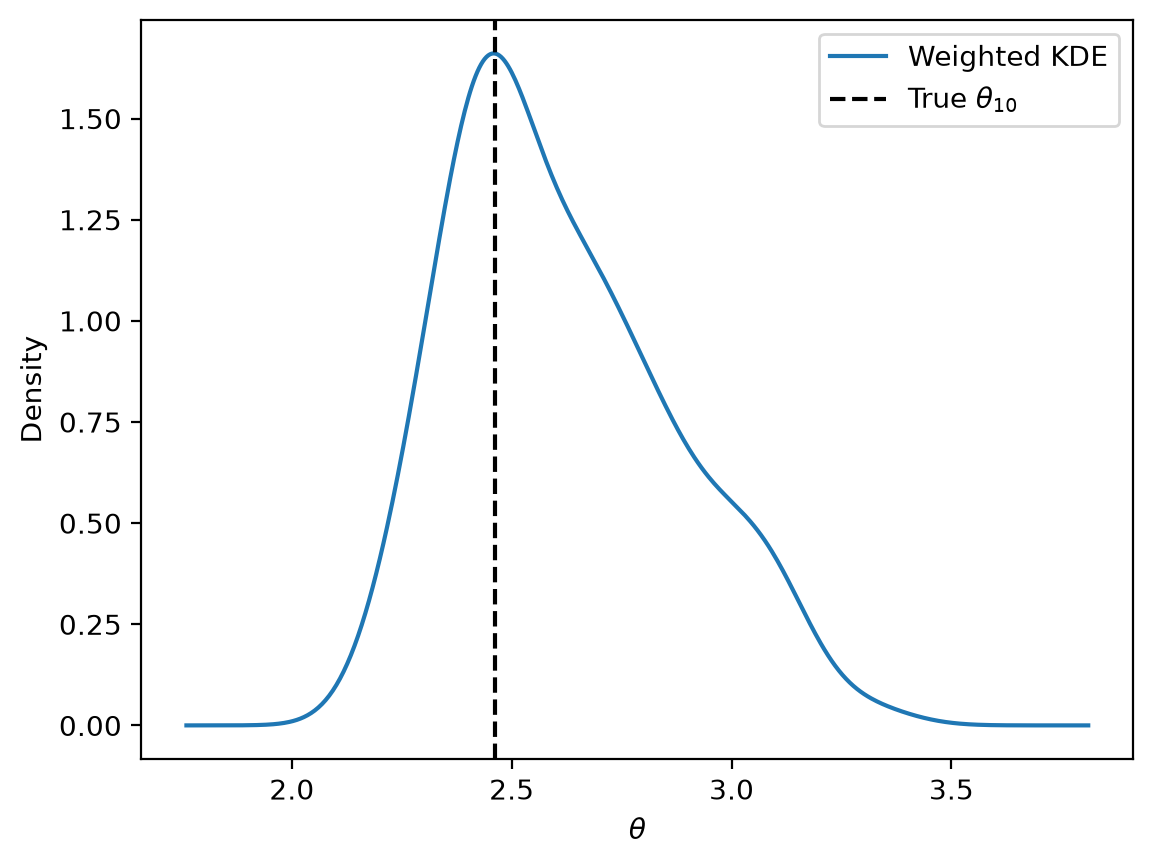
\includegraphics[width=\linewidth]{code/simulation/figures/penkf_filtering_theta.png}
        \caption{PEnKF}
    \end{subfigure}
    \hfill
    \begin{subfigure}{0.48\textwidth}
        \centering
        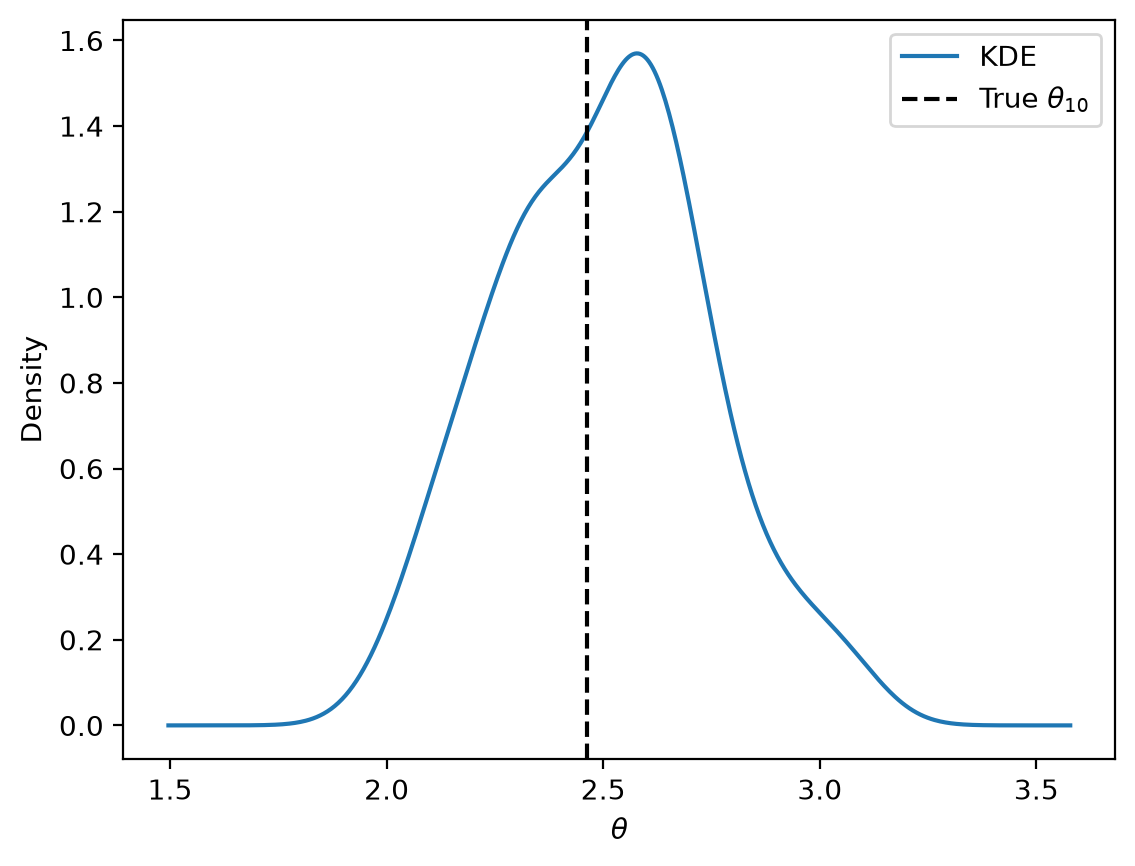
\includegraphics[width=\linewidth]{code/simulation/figures/genkf_filtering_theta.png}
        \caption{GEnKF}
    \end{subfigure}
    \caption{Filtering distribution of $\theta_{10}$ (kernel density estimate)
    against the true value.}
    \label{fig:filtering-theta}
\end{figure}

\clearpage % keep Appendix C's figure before this appendix
\section{Notation}\label{sec:notation}
Subscripts index time and coordinates, and superscripts index particles and
ensemble members. Bold lowercase letters are vectors, bold uppercase letters
are matrices, and the coordinates of a vector are plain, so $x_l$ is the $l$th
coordinate of $\vx$. Time subscripts are dropped in Appendix~\ref{sec:rainfall_appendix}, where the time
step is clear.

\renewcommand{\arraystretch}{1.15}
\begin{longtable}{@{}lp{0.78\textwidth}@{}}
\toprule
Symbol & Meaning \\
\midrule
\endhead
\multicolumn{2}{@{}l}{\emph{Sizes and indices}} \\
$d$ & Dimension of the latent state $\vx_t$ ($d = 100$ in the simulation study) \\
$m_t$ & Dimension of $\vy_t$ and $\vz_t$, the number of observation locations at time $t$ \\
$T$ & Number of time steps ($T = 10$) \\
$N$ & Number of particles: of $\theta$ in the PEnKF, and of $(\theta, \vx)$ in the particle filter \\
$M$ & Number of ensemble members: per $\theta$ particle in the PEnKF, and in total in the GEnKF \\
$t$ & Time step \\
$i$ & Particle index (superscript) \\
$j$ & Ensemble member index (superscript) \\
$l$ & Observation location (station) index \\
$\vz_{1:t}$ & All observations up to time $t$, $(\vz_1, \ldots, \vz_t)$ \\
\addlinespace
\multicolumn{2}{@{}l}{\emph{Model}} \\
$\theta_t$ & Scalar parameter; in the rainfall model, the power of the transformation from $\vy_t$ to $\vz_t$ \\
$\vx_t$ & Latent state; $x_l$ is its value at the $l$th observation location \\
$\tilde\vx_t$ & Forecast of the state, the propagated state before it is updated with $\vz_t$ \\
$\vy_t$ & Latent observations of the state with Gaussian noise, before the transformation \\
$\vz_t$ & Observed data, obtained by transforming $\vy_t$ \\
$\vu_t$ & Spatially correlated innovation of the AR(1) state model \\
$\mathcal M_t$ & Dynamics (forecast) model \\
$\mathbf Q_t$ & Covariance of the model noise in the dynamics \\
$\mathbf H_t$ & Observation matrix selecting the state at the observation locations \\
$\mathbf R_t$ & Covariance of the noise in $\vy_t$; $\mathbf R_t = \sigma_t^2\mathbf I_{m_t}$ in the rainfall model \\
$\sigma_t$ & Standard deviation of the observation noise ($\sigma_t = 0.2$) \\
$f_t$ & Density of the transformation from $\vy_t$ to $\vz_t$ \\
$\boldsymbol\mu_{0|0}$, $\mathbf\Sigma_{0|0}$ & Mean and covariance of the prior on $\vx_0$ \\
\addlinespace
\multicolumn{2}{@{}l}{\emph{Algorithms}} \\
$w^i$, $w^i_t$ & Normalized weight of particle $i$ (at time $t$) \\
$q_t$, $q$ & Proposal distributions: for $\theta_t$ in the PEnKF, and for $\vx^i_t$ in the proposed extension \\
$\boldsymbol\mu^i$, $\mathbf\Sigma^i$ & Mean and covariance of the proposal for $\vx^i_t$ in the proposed extension \\
$\mathcal L$ & Likelihood of the observations, with respect to the mixed measure $\nu$ \\
$\boldsymbol\mu$ & Mean of the forecast ensemble; $\mu_l$ is its $l$th coordinate \\
$\tilde{\mathbf\Sigma}$ & Covariance of the forecast ensemble \\
$\widehat{\mathbf\Sigma}$ & Approximate forecast covariance, $\tilde{\mathbf\Sigma} + \mathbf Q$ \\
$s_l^2$ & The $l$th diagonal entry of $\tilde{\mathbf\Sigma} + \mathbf Q$ \\
$\mathbf K$ & EnKF gain matrix \\
$\text{ESS}$ & Importance sampling effective sample size, $1 / \sum_{i=1}^N (w^i)^2$ \\
\addlinespace
\multicolumn{2}{@{}l}{\emph{Evaluation}} \\
$\widehat\vx$ & Posterior mean of the state (the weighted mean of the particles); $\widehat x_l$ is its $l$th coordinate \\
$F$ & CDF of a forecast distribution of one coordinate of $\vx$ \\
$X$, $X'$ & Independent draws from $F$ \\
$\text{RMSPE}$ & Root mean squared prediction error of $\widehat\vx$, averaged over the $d$ coordinates \\
$\text{CRPS}(F, x)$ & Continuous ranked probability score of $F$ at the true value $x$ \\
\addlinespace
\multicolumn{2}{@{}l}{\emph{Distributions and functions}} \\
$p(\cdot)$ & Generic density; $p(\cdot \mid \cdot)$ is a conditional density \\
$\Norm_k(\boldsymbol\mu, \mathbf\Sigma)$ & $k$-variate normal distribution; $\Norm_k(\vx; \boldsymbol\mu, \mathbf\Sigma)$ is its density at $\vx$. The subscript is omitted for scalars \\
$\Phi$ & Standard normal cumulative distribution function \\
$\text{Gamma}(a, b)$ & Gamma distribution with shape $a$ and rate $b$ \\
$\1_A$ & Indicator of the event $A$ \\
$\E$, $\P$ & Expectation and probability \\
$\lambda$, $\delta_0$ & Lebesgue measure, and Dirac delta measure at $0$ \\
$\nu$ & Dominating measure for the observations, $(\lambda + \delta_0)^{\otimes m}$ \\
\bottomrule
\end{longtable}

\begin{longtable}{@{}lp{0.78\textwidth}@{}}
\toprule
Abbreviation & Meaning \\
\midrule
\endhead
AR(1) & First-order autoregressive \\
CRPS & Continuous ranked probability score \\
EnKF & Ensemble Kalman filter \\
ESS & Effective sample size \\
FCD & Full conditional distribution \\
GEnKF & Gibbs ensemble Kalman filter \\
HMC & Hamiltonian Monte Carlo \\
HSSM & Hierarchical state-space model \\
MCMC & Markov chain Monte Carlo \\
PEnKF & Particle ensemble Kalman filter \\
RMSPE & Root mean squared prediction error \\
SMC & Sequential Monte Carlo \\
\bottomrule
\end{longtable}

\section{RMSPE and CRPS}\label{sec:metrics}
The RMSPE is based on the posterior mean and is averaged over space. That is,
given the true state $\vx$ and the posterior mean $\widehat\vx$ (the weighted
mean of the particles), we use
\begin{align}
    \text{RMSPE} = \sqrt{\frac 1 d \sum_{l=1}^d (x_l - \widehat x_l)^2}.
\end{align}
The CRPS measures the squared $L^2$ distance between the CDF of the predictive
distribution and the ideal CDF, which places a point mass at the true value.
That is, for one variable, denoting by $F$ the CDF of the forecast
distribution and by $x$ the true value
\begin{align}
    \text{CRPS}(F, x) &= \int_{-\infty}^{\infty} \left(F(u) - \1_{\{u \geq x\}}\right)^2 du.
\end{align}
This has an equivalent form \cite{gneiting2007}
\begin{align}
    \text{CRPS}(F, x) &= \E|X - x| - \frac 1 2 \E|X - X'|,
\end{align}
where $X$ and $X'$ are independent draws from $F$. This form can be evaluated
from samples. To get our overall CRPS score, we compute the CRPS score for each
dimension separately and then average the CRPS over the $d$ coordinates. The
code for this is based on the implementation in \cite{katzfuss2020}.

\end{document}